\documentclass[11pt, a4paper]{report}
%----------------------------------------------------------------------------------------
%	PACKAGES (宏包管理)
%----------------------------------------------------------------------------------------
% 1. 编码与语言
\usepackage[english]{babel}
\usepackage[T1]{fontenc}
% 2. 页面布局与排版
\usepackage{geometry}
\geometry{
    textwidth=6in, % 稍微加宽以便放入更好的box
    top=1in,
    bottom=1in,
    headheight=12pt,
    headsep=25pt,
    footskip=30pt
}
\usepackage{setspace}
\setstretch{1.2}
\usepackage{float}
\usepackage{enumitem} % 更好的列表控制
\usepackage{tocloft}  % 加载目录控制宏包
\renewcommand{\cftsecleader}{\cftdotfill{\cftdotsep}} % 强制让 section 后面显示点号
% 3. 数学支持
\usepackage{amsmath, amsthm, amssymb, amsfonts}
\usepackage{mathtools}
\usepackage{thmtools} % 定理环境增强
\usepackage{extarrows}
% 4. 图形与颜色
\usepackage{graphicx}
\usepackage[dvipsnames, svgnames]{xcolor} % 加载更多颜色名
\usepackage{tikz}
\usepackage{tikz-cd}
\usepackage{ytableau} % 杨表
\usetikzlibrary{decorations.pathreplacing, calc, shadows}

% Define reusable graph styles (The "Skill")
\tikzset{
    vertex/.style={circle, fill=black, inner sep=1.5pt, outer sep=0pt},
    graphlabel/.style={align=center, font=\small}
}

% 5. 漂亮的文本框
\usepackage{tcolorbox}
\tcbuselibrary{breakable, skins, theorems}
% 6. 参考文献
%\usepackage[backend=biber,style=gb7714-2015,sorting=gb7714-2015]{biblatex}
%\addbibresource{references.bib}
% 7. 交互 (最后加载)
\usepackage[hidelinks]{hyperref}
\usepackage{array}
%----------------------------------------------------------------------------------------
%	CUSTOM COLORS (自定义配色方案)
%----------------------------------------------------------------------------------------
% 定理色系 - 蓝色
\definecolor{ThmColor}{RGB}{0, 71, 171}        % 深钴蓝
\definecolor{ThmBg}{RGB}{240, 244, 255}        % 极浅蓝
% 定义色系 - 绿色
\definecolor{DefColor}{RGB}{0, 100, 0}         % 深绿
\definecolor{DefBg}{RGB}{240, 255, 240}        % 蜜瓜绿
% 引理/命题色系 - 橙色
\definecolor{LemColor}{RGB}{204, 85, 0}        % 焦橙色
\definecolor{LemBg}{RGB}{255, 248, 240}        % 极浅橙
% 示例/注记色系 - 灰色/紫色
\definecolor{ExColor}{RGB}{105, 105, 105}      % 暗灰
\definecolor{ExBg}{RGB}{250, 250, 250}         % 极浅灰
% 专题/话题色系 - 靛紫色
\definecolor{TopicColor}{RGB}{75, 0, 130}      % 靛蓝色 (Indigo)
\definecolor{TopicBg}{RGB}{248, 245, 255}      % 极浅紫
%----------------------------------------------------------------------------------------
%	THEOREM ENVIRONMENTS (环境美化核心)
%----------------------------------------------------------------------------------------
% 1. Theorem (蓝色风格)
\declaretheorem[name=Theorem, numberwithin=section]{theorem}
\tcolorboxenvironment{theorem}{
    enhanced jigsaw,
    colframe=ThmColor,       % 边框颜色
    colback=ThmBg,           % 背景颜色
    coltitle=white,          
    boxrule=0.5pt,           % 边框粗细
    leftrule=2pt,            % 左边框加粗
    sharp corners=downhill,  % 样式
    breakable,               % 允许跨页
    drop shadow=black!5!white % 轻微阴影
}
% Corollary 使用与 Theorem 相同的风格，但通常紧随其后
\declaretheorem[name=Corollary, numberlike=theorem]{corollary}
\tcolorboxenvironment{corollary}{
    enhanced jigsaw,
    colframe=ThmColor!80!white, 
    colback=ThmBg,
    boxrule=0pt, leftrule=2pt, arc=0pt, outer arc=0pt,
    breakable
}
% 2. Definition (绿色风格)
\declaretheorem[name=Definition, numberlike=theorem]{definition}
\tcolorboxenvironment{definition}{
    enhanced jigsaw,
    colframe=DefColor,
    colback=DefBg,
    boxrule=0.5pt, leftrule=2pt,
    sharp corners=downhill,
    breakable,
    drop shadow=black!5!white
}
% 3. Lemma & Proposition (橙色风格)
\declaretheorem[name=Lemma, numberlike=theorem]{lemma}
\declaretheorem[name=Proposition, numberlike=theorem]{proposition}
\tcolorboxenvironment{lemma}{
    enhanced jigsaw,
    colframe=LemColor,
    colback=LemBg,
    boxrule=0.5pt, leftrule=2pt,
    breakable
}
\tcolorboxenvironment{proposition}{
    enhanced jigsaw,
    colframe=LemColor,
    colback=LemBg,
    boxrule=0.5pt, leftrule=2pt
    % Keep propositions on one page to avoid zero-height first-part warnings
    % when a short box starts too close to a page break.
}
% 4. Example & Remark (简约风格)
\declaretheorem[name=Example, numberlike=theorem]{example}
\declaretheorem[name=Remark, numberlike=theorem]{remark}
\declaretheorem[name=Exercise, numberlike=theorem]{exercise}
\tcolorboxenvironment{example}{
    enhanced jigsaw,
    colframe=ExColor,
    colback=ExBg,
    leftrule=2pt, boxrule=0pt,
    frame hidden, % 隐藏其他三边
    breakable
}
% 5. Topic (靛紫色风格，带标题支持)
\declaretheorem[name=Topic, numberlike=theorem]{topic}
\tcolorboxenvironment{topic}{
    enhanced jigsaw,
    breakable,
    colframe=TopicColor,        % 边框为靛紫色
    colback=TopicBg,           % 背景为极浅紫
    boxrule=0.5pt,             % 细边框
    leftrule=2pt,              % 左侧加粗线
    sharp corners=downhill,    % 与你其他环境一致的切角样式
    drop shadow=black!5!white, % 轻微阴影
    before skip=15pt,
    after skip=15pt
}
%----------------------------------------------------------------------------------------
%	MATH MACROS (保留你的常用定义)
%----------------------------------------------------------------------------------------
\newcommand{\g}{\mathfrak{g}}  
\newcommand{\der}{\mathrm{d}} 
\newcommand{\h}{\mathfrak{h}} 
\newcommand{\n}{\mathfrak{n}}  
\newcommand{\U}{\mathcal{U}}  
\newcommand{\C}{\mathbb{C}} 
\newcommand{\R}{\mathbb{R}} 
\newcommand{\borel}{\mathfrak{b}}
\newcommand{\Ind}{\mathrm{Ind}} 
\newcommand{\Hom}{\mathrm{Hom}}  
\newcommand{\Ext}{\mathrm{Ext}}
\newcommand{\HRule}[1]{\rule{\linewidth}{#1}}
%----------------------------------------------------------------------------------------
%	TITLE PAGE
%----------------------------------------------------------------------------------------
\begin{document}
\hypersetup{pageanchor=false}
\begin{titlepage}
    \centering
    \vspace*{2cm}
    
    \textsc{\Large Course Notes}\\[0.5cm]

    \HRule{1.5pt} \\[0.5cm]
    { \huge \bfseries Combinatorics II }\\[0.4cm] 
    \HRule{1.5pt} \\[1.5cm]
    
    \vspace{3cm}

    % 人员信息区域：垂直排列并区分字号
    \begin{spacing}{1.8}
        {\Large \textbf{Instructor:}} \\
        {\Large Prof. Ferdinand \textsc{Ihringer}} \\[0.8cm]
        
        {\normalsize \textit{Student:}} \\
        {\normalsize Leo}
    \end{spacing}

    \vfill
    {\large \today}
\end{titlepage}
\hypersetup{pageanchor=true}
\newpage
\tableofcontents
\newpage


%----------------------------------------------------------------------------------------
%    CONTENT STRUCTURE TEMPLATE
%----------------------------------------------------------------------------------------
\chapter{Lecture 1}

\begin{tcolorbox}[
    enhanced,
    title=\textbf{Basic Information},
    colframe=TopicColor,
    colback=TopicBg,
    coltitle=white,
    boxrule=0.5pt,
    drop shadow=black!5!white,
    breakable
]
    \textbf{\textcolor{TopicColor}{Office hours:}} Mon, 13:45-15:45.
    
    \textbf{\textcolor{TopicColor}{Main book:}} \textit{A course in combinatorics} by J.H. van Lint and R.M. Wilson, 2nd edition. And the lecture notes by Prof. Ihringer.
    
    \textbf{\textcolor{TopicColor}{Grade:}} Final Exam: 40\%, midterm 30 \% (April 15, week 8 in class), Homework 20\%, Quizzes 10\% (very easy based on HW).
    
    \tcbline
    
    \textbf{\textcolor{TopicColor}{Homework:}} 
    \begin{itemize}[nosep, leftmargin=*]
        \item Biweekly
        \item Only handwritten on paper
        \item Submission in class
        \item Only in English
    \end{itemize}
    
    \tcbline
    
    \textbf{\textcolor{TopicColor}{Preliminary Schedule:}} 
    \begin{itemize}[nosep, leftmargin=*]
        \item \textbf{Week 1-4:} Basic graph theory, including trees, Ramsey numbers, Turan numbers, Hall's marriage theorem, etc.
        \item \textbf{Week 5-6:} Hadamard matrices.
        \item \textbf{Week 6-8:} Projective spaces.
        \item \textbf{Week 9:} Designs.
        \item \textbf{Week 10:} Strongly regular graphs.
        \item \textbf{Week 11:} Generalized Quadrangles.
        \item \textbf{Week 12-13:} General Spectral Graph Theory.
        \item \textbf{Week 14:} Associated Schemes.
        \item \textbf{Week 15:} Coding Theory.
    \end{itemize}
\end{tcolorbox}

\section{Introduction to Graphs}

\begin{definition}
A graph $G$ is a pair $(V, E)$ where $V$ is a set of vertices and $E$ is a set of edges.
\end{definition}

Let $G=(V,E)$ be a graph with vertex set $V$ and edge set $E$.

\begin{itemize}
\item If $G$ is directed, then edges are ordered pairs and $E\subseteq V\times V$;
\item If $G$ is simple undirected, then edges are unordered pairs and
$E\subseteq \binom{V}{2}$. (We call such $ G $ a normal graph in our course.)
\end{itemize}

\begin{definition}
    Let $G=(V,E)$ be a graph.
    \begin{itemize}
        \item Let $e=\{x,y\} \in E$. The vertices $x$ and $y$ are said to be \textbf{incident} with the edge $e$. Two vertices $x, y$ are called \textbf{adjacent} if $\{x,y\} \in E$.
        \item A vertex is called an \textbf{isolated vertex} if it is not incident with any edge.
        \item An edge connecting a vertex to itself is called a \textbf{loop}.
        \item Two or more edges connecting the same pair of vertices are called \textbf{multiple edges}.
    \end{itemize}
\end{definition}

\begin{example} 
    The following figure illustrates the definitions:
    \begin{center}
        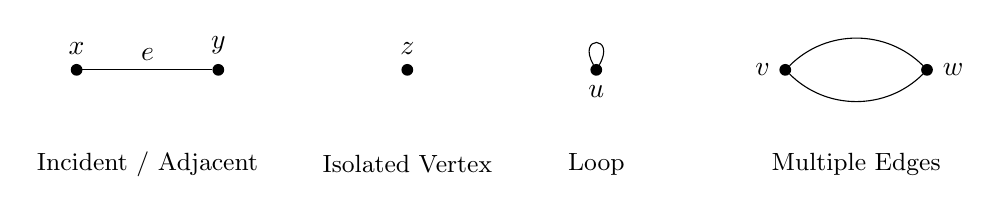
\begin{tikzpicture}[scale=1.2]
            % 1. Incident / Adjacent
            \node[vertex, label=above:$x$] (x) at (0,0) {};
            \node[vertex, label=above:$y$] (y) at (1.5,0) {};
            \draw (x) -- node[above] {$e$} (y);
            \node[graphlabel] at (0.75, -1) {Incident / Adjacent};

            % 2. Isolated Vertex
            \node[vertex, label=above:$z$] (z) at (3.5,0) {};
            \node[graphlabel] at (3.5, -1) {Isolated Vertex};

            % 3. Loop
            \node[vertex, label=below:$u$] (u) at (5.5,0) {};
            \draw (u) to [out=60,in=120,looseness=15] (u);
            \node[graphlabel] at (5.5, -1) {Loop};

            % 4. Multiple Edges
            \node[vertex, label=left:$v$] (v) at (7.5,0) {};
            \node[vertex, label=right:$w$] (w) at (9,0) {};
            \draw (v) to [bend left=45] (w);
            \draw (v) to [bend right=45] (w);
            \node[graphlabel] at (8.25, -1) {Multiple Edges};
        \end{tikzpicture}
    \end{center}
    \begin{itemize}
        \item \textbf{Incident/Adjacent}: Vertices $x$ and $y$ are adjacent and incident to edge $e$.
        \item \textbf{Isolated}: Vertex $z$ has no incident edges.
        \item \textbf{Loop}: Vertex $u$ has an edge connecting to itself.
        \item \textbf{Multiple Edges}: Vertices $v$ and $w$ are connected by two edges.
    \end{itemize}
\end{example}

\begin{definition}
    A graph is called a \textbf{planar graph} if it possesses a planar drawing, that is, it can be drawn in the plane such that no two edges intersect except at their endpoints.
\end{definition}

\begin{example} 
    Consider the following two drawings:
    \begin{center}
        \begin{tikzpicture}[scale=1]
            % ---------------- G_1 ----------------
            \coordinate (a1) at (90:1.6);
            \coordinate (b1) at (162:1.6);
            \coordinate (c1) at (234:1.6);
            \coordinate (d1) at (306:1.6);
            \coordinate (e1) at (18:1.6);
            \coordinate (f1) at (0,0.30);

            \draw (b1) -- (a1) -- (e1) -- (d1) -- (c1) -- (b1);
            \draw (a1) -- (f1) -- (c1);
            \draw (f1) -- (d1);

            \foreach \v in {a1,b1,c1,d1,e1,f1}
                \node[vertex] at (\v) {};

            \node at (0,-2.15) {$G_1$};

            % ---------------- G_2 ----------------
            \begin{scope}[xshift=7.8cm]
                \coordinate (a2) at (0,2.0);
                \coordinate (b2) at (-1.1,1.0);
                \coordinate (c2) at (1.1,1.0);
                \coordinate (d2) at (-1.1,-0.55);
                \coordinate (e2) at (1.1,-0.55);
                \coordinate (f2) at (0,-1.70);

                \draw (b2) -- (a2) -- (c2);
                \draw (b2) -- (d2);
                \draw (c2) -- (e2);
                \draw (d2) -- (e2);
                \draw (a2) -- (f2);
                \draw (d2) -- (f2) -- (e2);

                \foreach \v in {a2,b2,c2,d2,e2,f2}
                    \node[vertex] at (\v) {};

                \node at (0,-2.15) {$G_2$};
            \end{scope}
        \end{tikzpicture}
    \end{center}
$ G_1 $ and $ G_2 $ are \textbf{isomorphic}: If we pull the center node of $ G_1 $ then we get $ G_2 $. $ G_1 $ is planar, but $ G_2 $ is not. We call $ G_1 $ the plannar drawing of $ G_2 $, which means that $ G_1 $ has no edges intersect.     
\end{example}

\begin{definition} 
A graph without loops and multiple edges is called a \textbf{simple graph}.
\end{definition}

\begin{remark}
In the two statements above, the intended notion is essentially the same.
The condition ``$G$ is simple undirected'' together with
$E\subseteq \binom{V}{2}$ means that every edge is an unordered pair
$\{u,v\}$ of \emph{distinct} vertices, so loops are excluded automatically,
and since $E$ is a set (rather than a multiset), multiple edges are excluded
as well. Hence this coincides with the standard definition: a \emph{simple
graph} is a graph with no loops and no multiple edges.

In our course notes, such graphs are called \emph{normal graphs}. The only
minor caveat is that some texts use ``simple graph'' with the convention
that graphs are undirected by default, whereas others may state
``simple undirected'' explicitly. In the present context, these conventions
agree.
\end{remark}

\noindent \textbf{Convention: All our graphs are simple. Unless we say otherwise.}

\begin{definition}[Map coloring and the associated graph]
A \emph{map} (on the plane or on the sphere) is a decomposition of the surface
into finitely many regions (``countries'') such that any two regions meet
either in a boundary arc, in finitely many boundary points, or not at all.
Two countries are said to be \emph{adjacent} if they share a boundary segment
of positive length (meeting at a single point does \emph{not} count).

Given such a map, we define its \emph{adjacency graph} (also called the
\emph{dual graph}) $G=(V,E)$ as follows:
\[
V=\{\text{countries of the map}\},\qquad 
\{u,v\}\in E \iff \text{countries $u$ and $v$ are adjacent}.
\]
\end{definition}

\begin{remark}[Planarity]
The adjacency graph $G$ is \emph{planar}: it can be drawn in the plane with
no edge crossings by placing a vertex inside each country and drawing an edge
between two vertices through the common boundary segment of the corresponding
countries. Thus the problem of coloring maps is equivalent to coloring planar
graphs.
\end{remark}

\begin{definition}[Vertex coloring and chromatic number]
Let $G=(V,E)$ be a graph. A \emph{(proper) vertex coloring} of $G$ with $k$
colors is a map $c:V\to\{1,2,\dots,k\}$ such that
\[
\{u,v\}\in E \implies c(u)\neq c(v).
\]
The smallest $k$ for which such a coloring exists is called the
\emph{chromatic number} of $G$ and is denoted by $\chi(G)$.
\end{definition}

\begin{theorem}[Four-Color Theorem]
For every planar graph $G$, one has
\[
\chi(G)\le 4.
\]
Equivalently, every planar map can be colored with at most four colors so
that any two adjacent countries receive different colors.
\end{theorem}

\begin{remark}[Why ``at most 5 colors'' is easy]
A classical result (the \emph{Five-Color Theorem}) states that every planar
graph satisfies $\chi(G)\le 5$. This theorem admits a relatively short proof
using standard planar graph tools such as Euler's formula and a reducible
configuration argument (often presented via induction on $|V|$).
By contrast, the Four-Color Theorem is substantially deeper and historically
required extensive case-checking (computer-assisted) in its first proofs.
\end{remark}

The following statements are equivalent:
\[ \{ x,y \} \in E  \Leftrightarrow x \sim y \Leftrightarrow x,y \text{ adjacent } \Leftrightarrow x,y \text{ are neighbors}\]

\begin{example} 
$ |V|=n $, $ E=\binom{V}{2} $. Complete graph $ K_n $.

    \begin{center}
        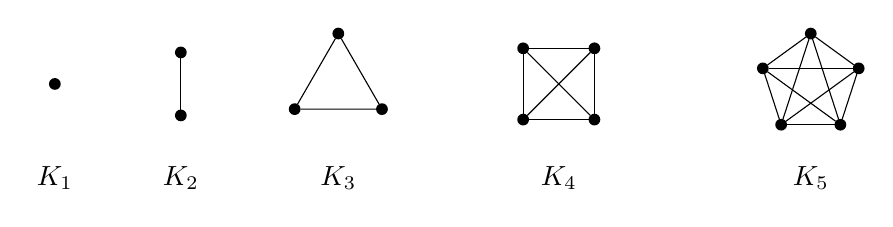
\begin{tikzpicture}[scale=0.8]
            % K_1
            \begin{scope}[shift={(0,0)}]
                \node[vertex] at (0,0) {};
                \node at (0,-1.5) {$K_1$};
            \end{scope}

            % K_2
            \begin{scope}[shift={(2,0)}]
                \node[vertex] (v1) at (0,0.5) {};
                \node[vertex] (v2) at (0,-0.5) {};
                \draw (v1) -- (v2);
                \node at (0,-1.5) {$K_2$};
            \end{scope}

            % K_3
            \begin{scope}[shift={(4.5,0)}]
                \foreach \i in {1,2,3}
                    \node[vertex] (v\i) at ({90 + (\i-1)*120}:0.8) {};
                \draw (v1) -- (v2) -- (v3) -- (v1);
                \node at (0,-1.5) {$K_3$};
            \end{scope}

            % K_4
            \begin{scope}[shift={(8,0)}]
                \foreach \i in {1,...,4}
                    \node[vertex] (v\i) at ({45 + (\i-1)*90}:0.8) {};
                \foreach \i in {1,...,4}
                    \foreach \j in {\i,...,4} {
                        \ifnum\i<\j \draw (v\i) -- (v\j); \fi
                    }
                \node at (0,-1.5) {$K_4$};
            \end{scope}

            % K_5
            \begin{scope}[shift={(12,0)}]
                \foreach \i in {1,...,5}
                    \node[vertex] (v\i) at ({90 + (\i-1)*72}:0.8) {};
                \foreach \i in {1,...,5}
                    \foreach \j in {\i,...,5} {
                        \ifnum\i<\j \draw (v\i) -- (v\j); \fi
                    }
                \node at (0,-1.5) {$K_5$};
            \end{scope}
        \end{tikzpicture}
    \end{center}
Remark: $ K_4 $ is a planar graph, but $ K_5 $ is not. 
    \begin{center}
        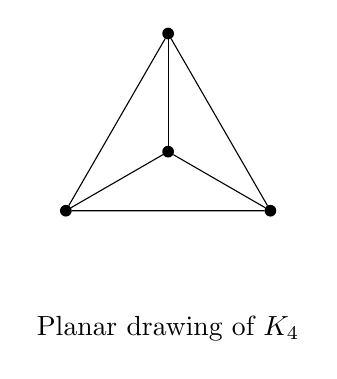
\begin{tikzpicture}[scale=1.5]
            \node[vertex] (v1) at (90:1) {};
            \node[vertex] (v2) at (210:1) {};
            \node[vertex] (v3) at (330:1) {};
            \node[vertex] (v4) at (0,0) {};
            
            \draw (v1) -- (v2) -- (v3) -- (v1);
            \draw (v4) -- (v1);
            \draw (v4) -- (v2);
            \draw (v4) -- (v3);
            
            \node at (0,-1.5) {Planar drawing of $K_4$};
        \end{tikzpicture}
    \end{center}
\end{example}

\begin{example} 
$ G=(V_1 \cup V_2, E) $ is bipartite if $ E \cap (\binom{V_1}{2} \cup \binom{V_2}{2}  )=\emptyset $.
    \begin{center}
        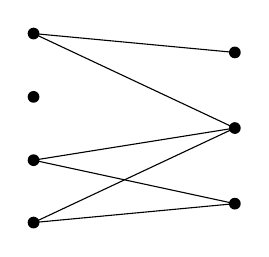
\begin{tikzpicture}[scale=1.2]
            % left part V_1 (one isolated vertex)
            \coordinate (l1) at (0,1.47);
            \coordinate (l2) at (0,0.80);
            \coordinate (l3) at (0,0.13);
            \coordinate (l4) at (0,-0.53);

            % right part V_2
            \coordinate (r1) at (2.13,1.27);
            \coordinate (r2) at (2.13,0.47);
            \coordinate (r3) at (2.13,-0.33);

            % edges
            \draw (l1) -- (r1);
            \draw (l1) -- (r2);
            \draw (l3) -- (r2);
            \draw (l3) -- (r3);
            \draw (l4) -- (r2);
            \draw (l4) -- (r3);

            % vertices
            \foreach \v in {l1,l2,l3,l4,r1,r2,r3}
                \node[vertex] at (\v) {};
        \end{tikzpicture}
    \end{center}
\end{example}

\begin{example} 
If $ E=\{ \{x,y\}: x \in V_1, y \in V_2 \} $, then $ G $ is a complete bipartite graph, denoted by $ K_{m,n} $ where $ m=|V_1|, n=|V_2| $.
    \begin{center}
        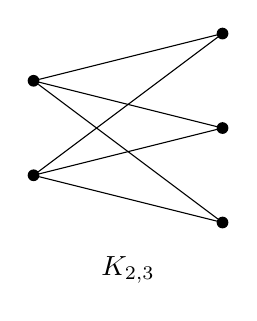
\begin{tikzpicture}[scale=1.2]
            % V_1 (size 2)
            \node[vertex] (u1) at (0, 0.5) {};
            \node[vertex] (u2) at (0, -0.5) {};
            
            % V_2 (size 3)
            \node[vertex] (v1) at (2, 1) {};
            \node[vertex] (v2) at (2, 0) {};
            \node[vertex] (v3) at (2, -1) {};
            
            % Edges
            \foreach \i in {1,2}
                \foreach \j in {1,2,3}
                    \draw (u\i) -- (v\j);
            
            \node at (1, -1.5) {$K_{2,3}$};
        \end{tikzpicture}
    \end{center}
\end{example}

\begin{example} 
Similarly we can define $ k $-partite graphs and complete $ k $-partite graphs.  

    \begin{center}
        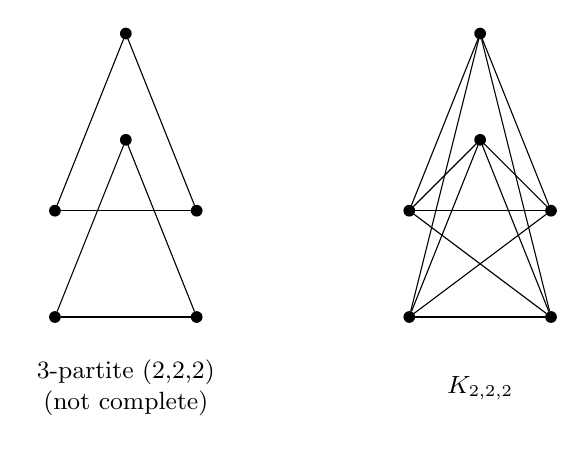
\begin{tikzpicture}[scale=0.9]
            % 3-partite (2,2,2) not complete
            \begin{scope}[shift={(0,0)}]
                \node[vertex] (a1) at (0,0) {}; \node[vertex] (a2) at (0,1.5) {};
                \node[vertex] (b1) at (2,0) {}; \node[vertex] (b2) at (2,1.5) {};
                \node[vertex] (c1) at (1,2.5) {}; \node[vertex] (c2) at (1,4) {};
                
                \draw (a1) -- (b1); \draw (a2) -- (b2);
                \draw (b1) -- (c1); \draw (b2) -- (c2);
                \draw (c1) -- (a1); \draw (c2) -- (a2);
                
                \node[graphlabel] at (1, -1) {3-partite (2,2,2) \\ (not complete)};
            \end{scope}

            % K_{2,2,2}
            \begin{scope}[shift={(5,0)}]
                \node[vertex] (u1) at (0,0) {}; \node[vertex] (u2) at (0,1.5) {};
                \node[vertex] (v1) at (2,0) {}; \node[vertex] (v2) at (2,1.5) {};
                \node[vertex] (w1) at (1,2.5) {}; \node[vertex] (w2) at (1,4) {};
                
                \foreach \i in {1,2} \foreach \j in {1,2} {
                    \draw (u\i) -- (v\j);
                    \draw (v\i) -- (w\j);
                    \draw (w\i) -- (u\j);
                }
                
                \node[graphlabel] at (1, -1) {$K_{2,2,2}$};
            \end{scope}
        \end{tikzpicture}
    \end{center}
\end{example}

\begin{example} 
The \textbf{$n$-dimensional hypercube} $Q_n$ is the graph with vertex set $V(Q_n) = \{0,1\}^n$, the set of binary strings of length $n$. Two vertices $x, y \in V(Q_n)$ are adjacent if and only if they differ in exactly one coordinate (i.e., their Hamming distance is $1$). The graph $Q_n$ is $n$-regular with $|V(Q_n)|=2^n$ and $|E(Q_n)|=n2^{n-1}$. For $n=3$, we have $110 \sim 111$, whereas $111 \nsim 100$.

    \begin{center}
        \begin{tikzpicture}[scale=0.85]
            % Q_0
            \begin{scope}[shift={(0,0)}]
                \node[vertex,label=above:$\emptyset$] (q00) at (0,0) {};
                \node[graphlabel] at (0,-1.2) {$Q_0$};
            \end{scope}

            % Q_1
            \begin{scope}[shift={(4.5,0)}]
                \node[vertex,label=above:$0$] (q10) at (0,0) {};
                \node[vertex,label=above:$1$] (q11) at (1.8,0) {};
                \draw (q10) -- (q11);
                \node[graphlabel] at (0.9,-1.2) {$Q_1$};
            \end{scope}

            % Q_2
            \begin{scope}[shift={(9.5,0)}]
                \node[vertex,label=left:$00$]  (a) at (0,0) {};
                \node[vertex,label=right:$10$] (b) at (2,0) {};
                \node[vertex,label=left:$01$]  (c) at (0,2) {};
                \node[vertex,label=right:$11$] (d) at (2,2) {};
                \draw (a) -- (b) -- (d) -- (c) -- (a);
                \node[graphlabel] at (1,-1.2) {$Q_2$};
            \end{scope}

            % Q_3
            \begin{scope}[shift={(4.25,-5.5)}]
                % front square (last bit = 0)
                \node[vertex,label=left:$000$]  (f1) at (0,0) {};
                \node[vertex,label=right:$100$] (f2) at (2,0) {};
                \node[vertex,label=left:$010$]  (f3) at (0,2) {};
                \node[vertex,label=right:$110$] (f4) at (2,2) {};
                \draw (f1) -- (f2) -- (f4) -- (f3) -- (f1);

                % back square (last bit = 1)
                \node[vertex,label=left:$001$]  (b1) at (1,0.8) {};
                \node[vertex,label=right:$101$] (b2) at (3,0.8) {};
                \node[vertex,label=left:$011$]  (b3) at (1,2.8) {};
                \node[vertex,label=right:$111$] (b4) at (3,2.8) {};
                \draw (b1) -- (b2) -- (b4) -- (b3) -- (b1);

                % connecting edges
                \draw (f1) -- (b1);
                \draw (f2) -- (b2);
                \draw (f3) -- (b3);
                \draw (f4) -- (b4);

                \node[graphlabel] at (1.5,-1.2) {$Q_3$};
            \end{scope}
        \end{tikzpicture}
    \end{center}
\end{example}

\begin{example} 
Let $S$ be a set with 3 elements, for instance $S=\{1,2,3\}$. The power set $\mathcal{P}(S)$ can be made into a graph by defining two subsets $A, B \subseteq S$ to be adjacent if their symmetric difference has size one, i.e., $|A \Delta B| = 1$. This graph is isomorphic to the 3-dimensional hypercube $Q_3$. The structure is often drawn as the Hasse diagram of the subset lattice.

    \begin{center}
        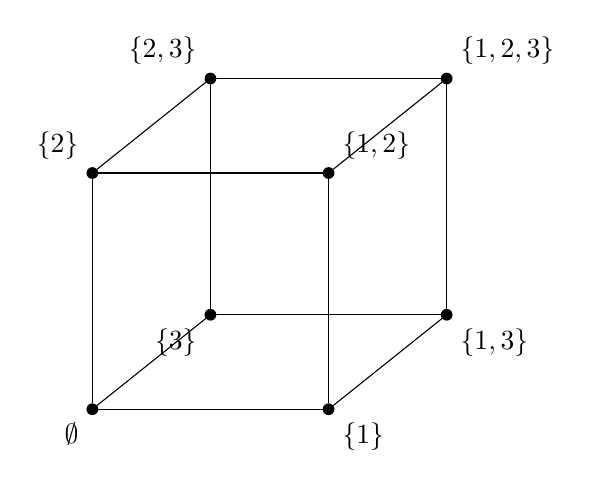
\begin{tikzpicture}[scale=1.5]
            % front square (subsets of {1,2})
            \node[vertex,label=below left:$\emptyset$]  (f1) at (0,0) {};
            \node[vertex,label=below right:$\{1\}$] (f2) at (2,0) {};
            \node[vertex,label=above left:$\{2\}$]  (f3) at (0,2) {};
            \node[vertex,label={above right:$\{1,2\}$}] (f4) at (2,2) {};
            \draw (f1) -- (f2) -- (f4) -- (f3) -- (f1);

            % back square (element 3 is added)
            \node[vertex,label=below left:$\{3\}$]  (b1) at (1,0.8) {};
            \node[vertex,label={below right:$\{1,3\}$}] (b2) at (3,0.8) {};
            \node[vertex,label={above left:$\{2,3\}$}]  (b3) at (1,2.8) {};
            \node[vertex,label={above right:$\{1,2,3\}$}] (b4) at (3,2.8) {};
            \draw (b1) -- (b2) -- (b4) -- (b3) -- (b1);

            % connecting edges
            \draw (f1) -- (b1);
            \draw (f2) -- (b2);
            \draw (f3) -- (b3);
            \draw (f4) -- (b4);
        \end{tikzpicture}
    \end{center}
    \begin{center}
        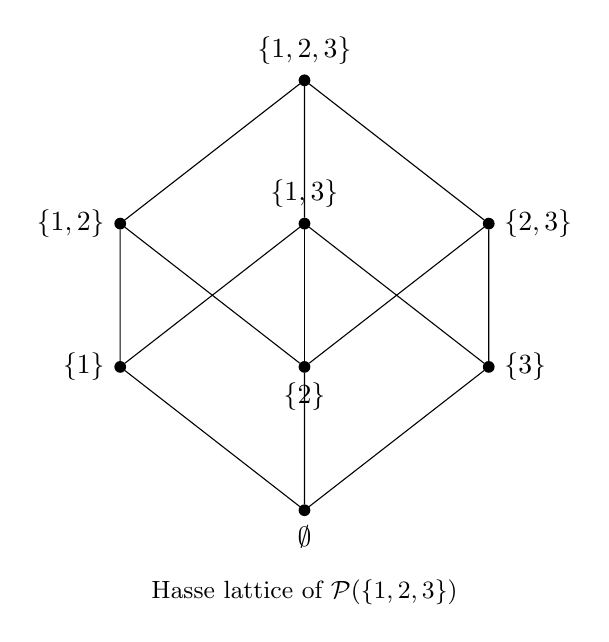
\begin{tikzpicture}[scale=1.3]
            % Boolean lattice B_3 (Hasse diagram of subsets of {1,2,3})
            \node[vertex,label=below:$\emptyset$] (e) at (0,0) {};

            \node[vertex,label={left:$\{1\}$}]  (a1) at (-1.8,1.4) {};
            \node[vertex,label={below:$\{2\}$}] (a2) at (0,1.4) {};
            \node[vertex,label={right:$\{3\}$}] (a3) at (1.8,1.4) {};

            \node[vertex,label={left:$\{1,2\}$}]  (b1) at (-1.8,2.8) {};
            \node[vertex,label={above:$\{1,3\}$}] (b2) at (0,2.8) {};
            \node[vertex,label={right:$\{2,3\}$}] (b3) at (1.8,2.8) {};

            \node[vertex,label={above:$\{1,2,3\}$}] (t) at (0,4.2) {};

            % cover relations
            \draw (e) -- (a1) -- (b1) -- (t);
            \draw (e) -- (a2) -- (b1);
            \draw (e) -- (a3) -- (b3) -- (t);
            \draw (a1) -- (b2) -- (t);
            \draw (a2) -- (b2);
            \draw (a2) -- (b3);
            \draw (a3) -- (b2);

            \node[graphlabel] at (0,-0.8) {Hasse lattice of $\mathcal{P}(\{1,2,3\})$};
        \end{tikzpicture}
    \end{center}
This graph is another representation of $Q_3$.
\end{example}

\begin{example} 
$ P_n $: path of length $ n-1 $.   

    \begin{center}
        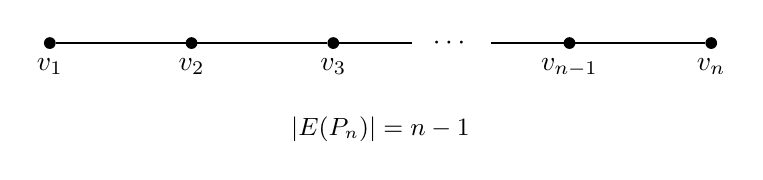
\begin{tikzpicture}[scale=1.0]
            \node[vertex,label=below:$v_1$] (v1) at (0,0) {};
            \node[vertex,label=below:$v_2$] (v2) at (1.8,0) {};
            \node[vertex,label=below:$v_3$] (v3) at (3.6,0) {};
            \node (dots) at (5.1,0) {$\cdots$};
            \node[vertex,label=below:$v_{n-1}$] (vnm1) at (6.6,0) {};
            \node[vertex,label=below:$v_n$] (vn) at (8.4,0) {};

            \draw (v1) -- (v2) -- (v3);
            \draw (v3) -- (4.6,0);
            \draw (5.6,0) -- (vnm1) -- (vn);

            \node[graphlabel] at (4.2,-1.1) {$|E(P_n)|=n-1$};
        \end{tikzpicture}
    \end{center}

\end{example}

\begin{example} 
With $ \{ v_n, v_1 \}  $ added, we get a cycle $ C_n $. For example $ C_6 $:
    \begin{center}
        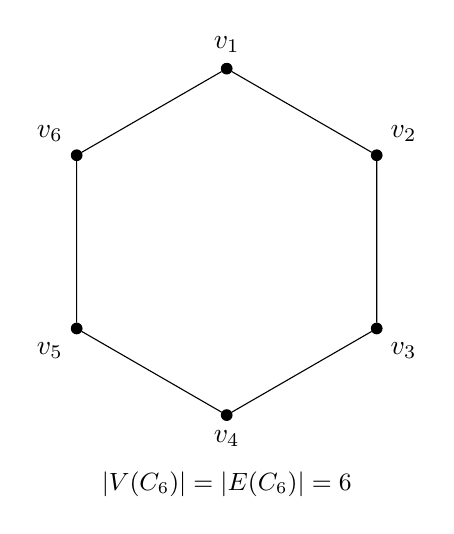
\begin{tikzpicture}[scale=1.1]
            \node[vertex,label=above:$v_1$] (v1) at (90:2) {};
            \node[vertex,label={above right:$v_2$}] (v2) at (30:2) {};
            \node[vertex,label={below right:$v_3$}] (v3) at (-30:2) {};
            \node[vertex,label=below:$v_4$] (v4) at (-90:2) {};
            \node[vertex,label={below left:$v_5$}] (v5) at (-150:2) {};
            \node[vertex,label={above left:$v_6$}] (v6) at (150:2) {};

            \draw (v1) -- (v2) -- (v3) -- (v4) -- (v5) -- (v6) -- (v1);

            \node[graphlabel] at (0,-2.8) {$|V(C_6)|=|E(C_6)|=6$};
        \end{tikzpicture}
    \end{center}


\end{example}

\begin{example} 
Peterson Graph: 
    \begin{center}
        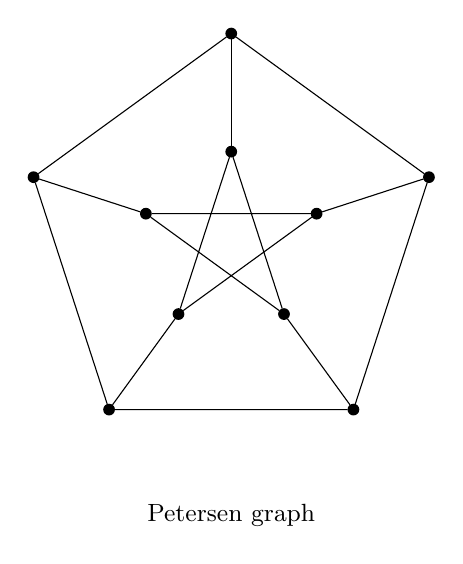
\begin{tikzpicture}[scale=1.2]
            % Outer 5-cycle
            \foreach \i in {1,...,5} {
                \node[vertex] (o\i) at (90-72*\i:2.2) {};
            }
            \draw (o1) -- (o2) -- (o3) -- (o4) -- (o5) -- (o1);

            % Inner pentagram
            \foreach \i in {1,...,5} {
                \node[vertex] (i\i) at (90-72*\i:0.95) {};
            }
            \draw (i1) -- (i3) -- (i5) -- (i2) -- (i4) -- (i1);

            % Spokes
            \foreach \i in {1,...,5} {
                \draw (o\i) -- (i\i);
            }

            \node[graphlabel] at (0,-2.9) {Petersen graph};
        \end{tikzpicture}
    \end{center}

Each vertix has degree 3 so this graph is $ 3 $-regular. Any two vertices linked by an edge has no common neighbor. Any 2 vertices not linked by an edge has a common neighbor.

It is a strongly regular graph with parameters $ (10,3,0,1) $.
\end{example}

\begin{definition}[Strongly regular graph]
Let $G=(V,E)$ be a simple undirected graph. We say that $G$ is \emph{strongly regular}
with parameters $(v,k,\lambda,\mu)$ if the following hold:
\begin{enumerate}
  \item $|V|=v$ and $G$ is $k$-regular (i.e.\ every vertex has degree $k$);
  \item for any two \emph{adjacent} vertices $x\sim y$, the number of common neighbors of $x$ and $y$
        is exactly $\lambda$, i.e.\ $|\Gamma(x)\cap \Gamma(y)|=\lambda$;
  \item for any two \emph{non-adjacent} vertices $x\not\sim y$, the number of common neighbors of $x$ and $y$
        is exactly $\mu$, i.e.\ $|\Gamma(x)\cap \Gamma(y)|=\mu$.
\end{enumerate}
\end{definition}

\begin{example} 
$ G=(V,E) $, $ \bar{G}=(V,\bar{E}) $, where $ \bar{E}=\binom{V}{2} \setminus E$. $ \bar{G} $ is the complement of $ G $.

    \begin{center}
        \begin{tikzpicture}[scale=1.0]
            % ---------- Top-left: G ----------
            \begin{scope}[shift={(0,0)}]
                \node[vertex] (a) at (0,2) {};
                \node[vertex] (b) at (2,2) {};
                \node[vertex] (c) at (0,0) {};
                \node[vertex] (d) at (2,0) {};

                \draw (a) -- (b);
                \draw (a) -- (c);
                \draw (b) -- (d);
                \draw (a) -- (d);

                \node[graphlabel] at (1,-1.1) {$G$};
            \end{scope}

            % ---------- Top-right: \bar{G} ----------
            \begin{scope}[shift={(7,0)}]
                \node[vertex] (e) at (0,2) {};   % isolated
                \node[vertex] (f) at (0,0) {};
                \node[vertex] (g) at (2,0) {};
                \node[vertex] (h) at (2,2) {};

                \draw (f) -- (g);
                \draw (f) -- (h);

                \node[graphlabel] at (1,-1.1) {$\overline{G}$};
            \end{scope}

            % ---------- Bottom-left: P_4 ----------
            \begin{scope}[shift={(0,-5.4)}]
                \node[vertex] (p1) at (0,2) {};
                \node[vertex] (p2) at (2,2) {};
                \node[vertex] (p3) at (0,0) {};
                \node[vertex] (p4) at (2,0) {};

                \draw (p3) -- (p1) -- (p2) -- (p4);

                \node[graphlabel] at (1,-1.1) {$P_4$};
            \end{scope}

            % ---------- Bottom-right: \overline{P_4} ----------
            \begin{scope}[shift={(7,-5.4)}]
                \node[vertex] (q1) at (0,2) {};
                \node[vertex] (q2) at (2,2) {};
                \node[vertex] (q3) at (0,0) {};
                \node[vertex] (q4) at (2,0) {};

                \draw (q1) -- (q4);
                \draw (q3) -- (q2);
                \draw (q3) -- (q4);

                \node[graphlabel] at (1,-1.1) {$\overline{P_4}$};
            \end{scope}
        \end{tikzpicture}
    \end{center}
In this example, observe that $ P_4 \cong \overline{P_4} $. We call such a graph self-complementary. A graph $G$ is self-complementary if $G \cong \overline{G}$. 
\end{example}

\begin{definition} 
Let $ G=(V,E) $ and $ G'=(V',E') $. They are isomorphic if and only if there exists a bijection $ \phi: V \to V' $ such that $ \{ x,y \} \in E \Leftrightarrow \{ \phi(x), \phi(y) \} \in E' $.
\end{definition}

\begin{definition} 
$ \sharp y : y \sim x =$ degree of $ x $, denoted by $ \deg(x) $ or $ \mathrm{d} (x)$. If $ \mathrm{d}(x) =\mathrm{d}(y)$ for all $ x,y \in V $, then $ G $ is $ d $-regular.
\end{definition}

\begin{remark}[Degree sequence: definition and uses]
Let $G=(V,E)$ be a simple undirected graph with $n=|V|$.  The \emph{degree sequence} of $G$
is the list of vertex degrees arranged in nonincreasing order,
\[
d_1 \ge d_2 \ge \cdots \ge d_n,
\qquad \text{where } \{d_1,\dots,d_n\}=\{\deg(v):v\in V\}.
\]

It is useful for:
\begin{itemize}
  \item \textbf{Coarse structural information:} by the Handshaking Lemma,
  $\sum_{i=1}^n d_i = 2|E|$, so the degree sequence determines the number of edges and
  reveals properties such as regularity (all $d_i$ equal).
  \item \textbf{Realizability tests:} deciding whether a given integer sequence is
  \emph{graphical} (i.e.\ occurs as the degree sequence of a simple graph), using
  criteria such as the Erd\H{o}s--Gallai theorem or the Havel--Hakimi algorithm
  (which can also construct a realizing graph).
  \item \textbf{Isomorphism invariant:} isomorphic graphs have the same degree sequence,
  so differing degree sequences imply non-isomorphism, though the converse need not hold.
  \item \textbf{Algorithmic and modeling input:} degree sequences serve as compact summaries
  in extremal graph theory, network models (e.g.\ random graphs with prescribed degrees),
  and matrix-based methods (e.g.\ Laplacian $L=D-A$ where $D$ is the degree matrix).
\end{itemize}
\end{remark} 

\begin{example} 
$ d_1=2,d_2=1,d_3=1 $. This graph is $ P_3 $.  
\end{example}

\begin{example} 
Consider the following 3 graphs:

\begin{center}
    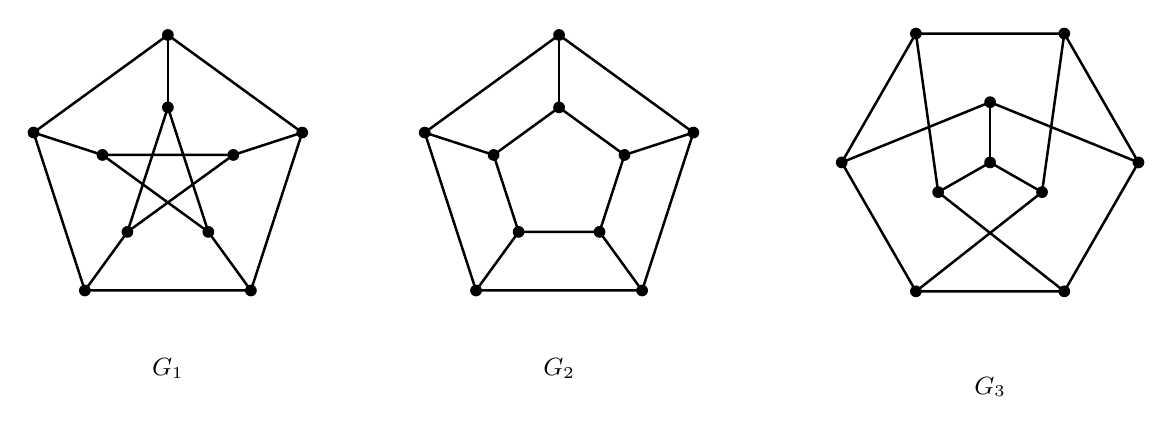
\begin{tikzpicture}[scale=0.92, every path/.style={line width=0.9pt}]
        % ---------------- G_1 ----------------
        \begin{scope}[xshift=0cm]
            % Use exactly the same 10-point layout as G_2
            \foreach \i in {1,...,5} {
                \coordinate (gOneO\i) at (90-72*\i:1.95);
                \coordinate (gOneI\i) at (90-72*\i:0.95);
            }

            % Outer 5-cycle
            \draw (gOneO1)--(gOneO2)--(gOneO3)--(gOneO4)--(gOneO5)--(gOneO1);

            % Spokes
            \foreach \i in {1,...,5} {
                \draw (gOneO\i)--(gOneI\i);
            }

            % Inner 5-point star (not pentagon)
            \draw (gOneI1)--(gOneI3)--(gOneI5)--(gOneI2)--(gOneI4)--(gOneI1);

            \foreach \p in {gOneO1,gOneO2,gOneO3,gOneO4,gOneO5,gOneI1,gOneI2,gOneI3,gOneI4,gOneI5} {
                \node[vertex] at (\p) {};
            }
            \node[graphlabel] at (0,-2.65) {$G_1$};
        \end{scope}

        % ---------------- G_2 ----------------
        \begin{scope}[xshift=5.4cm]
            % Outer pentagon
            \foreach \i in {1,...,5} {
                \coordinate (o\i) at (90-72*\i:1.95);
            }
            \draw (o1)--(o2)--(o3)--(o4)--(o5)--(o1);

            % Inner pentagon (parallel 5-cycle)
            \foreach \i in {1,...,5} {
                \coordinate (i\i) at (90-72*\i:0.95);
            }
            \draw (i1)--(i2)--(i3)--(i4)--(i5)--(i1);

            % Matching spokes
            \foreach \i in {1,...,5} {
                \draw (o\i)--(i\i);
            }

            \foreach \p in {o1,o2,o3,o4,o5,i1,i2,i3,i4,i5} {
                \node[vertex] at (\p) {};
            }
            \node[graphlabel] at (0,-2.65) {$G_2$};
        \end{scope}

        % ---------------- G_3 ----------------
        \begin{scope}[xshift=10.8cm, yshift=-0.26cm]
            % Uniformly enlarge the whole graph around its center (0.55,0.45)
            \begin{scope}[shift={(0.55,0.45)}, scale=1.28, shift={(-0.55,-0.45)}]
                % Layout matching the reference drawing
                \coordinate (gThreeA) at (-1.05, 0.45);  % left
                \coordinate (gThreeB) at (-0.25, 1.84);  % top-left
                \coordinate (gThreeC) at ( 1.35, 1.84);  % top-right
                \coordinate (gThreeD) at ( 2.15, 0.45);  % right
                \coordinate (gThreeE) at ( 1.35,-0.94);  % bottom-right
                \coordinate (gThreeF) at (-0.25,-0.94);  % bottom-left
                \coordinate (gThreeG) at ( 0.55, 1.10);  % inner triangle: top
                \coordinate (gThreeH) at ( 0.55, 0.45);  % graph center
                \coordinate (gThreeI) at (-0.01, 0.13);  % inner triangle: bottom-left
                \coordinate (gThreeJ) at ( 1.11, 0.13);  % inner triangle: bottom-right

                % Outer cycle
                \draw (gThreeB)--(gThreeC)--(gThreeD)--(gThreeE)--(gThreeF)--(gThreeA)--(gThreeB);

                % Inner/connecting edges
                \draw (gThreeA)--(gThreeG)--(gThreeD);
                \draw (gThreeB)--(gThreeI);
                \draw (gThreeC)--(gThreeJ);
                \draw (gThreeG)--(gThreeH);
                \draw (gThreeH)--(gThreeI);
                \draw (gThreeH)--(gThreeJ);
                \draw (gThreeI)--(gThreeE);
                \draw (gThreeJ)--(gThreeF);

                \foreach \p in {gThreeA,gThreeB,gThreeC,gThreeD,gThreeE,gThreeF,gThreeG,gThreeH,gThreeI,gThreeJ} {
                    \node[vertex] at (\p) {};
                }
            \end{scope}
            \node[graphlabel] at (0.55,-2.65) {$G_3$};
        \end{scope}
    \end{tikzpicture}
\end{center}

$ G_1 \ncong G_2 $, $ G_2 \ncong G_3 $, but $ G_1 \cong G_3 $.
\end{example}

The \emph{graph isomorphism problem} (GI) asks: given two finite graphs $G$ and $H$, decide whether there exists a bijection between their vertex sets that preserves adjacency (i.e.\ an isomorphism).  From the viewpoint of worst-case complexity, GI has long occupied an intermediate position: it is in $\mathrm{NP}$, but it is neither known to be $\mathrm{NP}$-complete nor known to admit a polynomial-time algorithm.  A major milestone is Babai's 2015 breakthrough, which gives a \emph{quasi-polynomial} time algorithm for GI, running in time $\exp\!\big((\log n)^{O(1)}\big)$ on $n$-vertex graphs, substantially improving the best previously known general upper bounds.

In parallel with the worst-case theory, there is a large body of \emph{practical} work aimed at solving typical instances efficiently, often via \emph{canonical labeling} and computation of automorphism groups.  Since the 1990s, McKay's software \texttt{nauty} (and later \texttt{Traces}, with further algorithmic refinements) has been highly effective on a wide range of graphs encountered in applications.  However, strong empirical performance does not settle the worst-case complexity question, and there exist carefully constructed families of graphs that can be difficult for certain refinement-and-search heuristics.  Thus, it is important to distinguish clearly between (i) the unresolved \emph{theoretical} question of whether GI is solvable in polynomial time in the worst case, and (ii) the largely successful but still evolving \emph{algorithm engineering} of fast GI solvers for real-world inputs.

\begin{proposition}[handshaking lemma]
$ G=(V,E) $. Then 
\[
\sum_{v \in V} \deg(v) = 2|E|
\]  
\end{proposition}

\begin{proof} 
Count $ (x,e) \in V \times E $ where $ x \in e $ in two ways. First, for each $ e \in E $, there are exactly two vertices $ x \in e $. So the number of such pairs is $ 2|E| $. Second, for each $ x \in V $, there are exactly $ \deg(x) $ edges $ e \in E $ containing $ x $. So the number of such pairs is $ \sum_{v \in V} \deg(v) $. Equating these two counts gives the desired result.
\end{proof}

\begin{theorem} 
A finite graph (we only talk about finite graphs in our class) has an even number of vertices with odd degree.
\end{theorem}

\begin{proof}
Consider
\[
\sum_{v\in V} \deg(v) = 2|E|,
\]
which is an even integer.

Reduce this congruence modulo $2$. Vertices of even degree contribute $0$ modulo $2$, and vertices of odd degree contribute $1$ modulo $2$. Hence
\[
\sum_{v\in V} \deg(v) \equiv \#\{v\in V:\deg(v)\ \text{is odd}\} \pmod{2}.
\]
Since the left-hand side is even, the right-hand side is $0 \pmod{2}$, so the number of odd-degree vertices is even.
\end{proof}

\begin{definition}[subgraph] 
Let $ G=(V,E) $ be a graph. A graph $ H=(V',E') $ is a \emph{subgraph} of $ G $ if $ V' \subseteq V $ and $ E' \subseteq E $. 
\end{definition}

\begin{definition}[induced subgraph] 
Let $ G=(V,E) $ be a graph. A graph $ H=(V',E') $ is an \emph{induced subgraph} of $ G $ if $ V' \subseteq V $ and $ E' = E \cap \binom{V'}{2} $. 
\end{definition}

\begin{example} 
Consider the graph $ K_4 $, we have two subgraph $C_3$ and $C_4$. The subgraph $C_3$ is an induced subgraph, but the subgraph $C_4$ is not.

\begin{center}
    \resizebox{0.94\textwidth}{!}{%
    \begin{tikzpicture}[scale=1.15]
        % K_4
        \begin{scope}[shift={(0,0)}]
            \coordinate (a) at (135:1);
            \coordinate (b) at (45:1);
            \coordinate (c) at (-45:1);
            \coordinate (d) at (-135:1);
            \draw (a) -- (b) -- (c) -- (d) -- (a);
            \draw (a) -- (c);
            \draw (b) -- (d);
            \foreach \p/\name/\pos in {a/1/above left,b/2/above right,c/3/below right,d/4/below left}
                \node[vertex, label={\pos:$v_{\name}$}] at (\p) {};
            \node at (0,-1.7) {$K_4$};
        \end{scope}

        % C_3 as an induced subgraph
        \begin{scope}[shift={(5.2,0)}]
            \coordinate (a) at (90:1);
            \coordinate (b) at (210:1);
            \coordinate (c) at (330:1);
            \draw (a) -- (b) -- (c) -- (a);
            \foreach \p/\name in {a/1,b/2,c/3}
                \node[vertex, label={\name*120-30:$v_{\name}$}] at (\p) {};
            \node at (0,-1.7) {$C_3$};
            \node[graphlabel] at (0,-2.35) {induced subgraph};
        \end{scope}

        % C_4 as a non-induced subgraph
        \begin{scope}[shift={(10.8,0)}]
            \coordinate (a) at (-1,1);
            \coordinate (b) at (1,1);
            \coordinate (c) at (1,-1);
            \coordinate (d) at (-1,-1);
            \draw (a) -- (b) -- (c) -- (d) -- (a);
            \foreach \p/\name/\pos in {a/1/above left,b/2/above right,c/3/below right,d/4/below left}
                \node[vertex, label={\pos:$v_{\name}$}] at (\p) {};
            \node at (0,-1.7) {$C_4$};
            \node[graphlabel] at (0,-2.35) {not induced in $K_4$};
        \end{scope}
    \end{tikzpicture}%
    }
\end{center}

For $C_3$, we choose the vertices $\{v_1,v_2,v_3\}$, and every edge among them in $K_4$ is kept, so it is induced. For $C_4$, we use all four vertices but delete the two diagonals, so it is a subgraph but not an induced subgraph.
\end{example}

\textbf{Adjacency list representation.}

Let $G=(V,E)$ be a (finite) graph with $V=\{1,2,\dots,n\}$.  In an \emph{adjacency list} representation, the computer stores an array (or map) $\mathrm{Adj}$ indexed by vertices, where $\mathrm{Adj}[u]$ is the list of all neighbors of $u$:
\[
\mathrm{Adj}[u]=\{\,v\in V : \{u,v\}\in E\,\}\quad\text{(undirected)}, \\
\mathrm{Adj}[u]=\{\,v\in V : (u,v)\in E\,\}\quad\text{(directed)}.
\]
For an undirected simple graph each edge $\{u,v\}$ appears twice, once in $\mathrm{Adj}[u]$ and once in $\mathrm{Adj}[v]$.  This data structure supports efficient traversal of neighbors (e.g.\ BFS/DFS) in total time $O(|V|+|E|)$ and uses space $O(|V|+|E|)$ for sparse graphs.

For our human beings we use the following matrices:

\begin{definition}[adjacent matrix] 
Let $ G=(V,E) $ be a graph. Let $V=\{v_1, v_2, \ldots, v_n\}$ and $E=\{e_1, e_2, \ldots, e_m\}$. Let $A=(a_{ij})$ where $a_{ij}=1$ if $v_i \sim v_j$, and $a_{ij}=0$ otherwise. Then $A$ is called the \emph{adjacent matrix} of $G$. For the base field usually we use $\mathbb{R}$, $\mathbb{C}$, $\mathbb{F}_2$, $\mathbb{F}_q$.
\end{definition}

\begin{remark}
In our class we mainly use consider $ A \in \mathbb{R}^{n \times n} $. Sometimes we will consider $ A \in \mathbb{C}^{n \times n} $ when we move to spectral graph theory.   
\end{remark}

\begin{definition}[Incidence matrix] 
Let $ B=(b_{ij}) $, $ B \in \mathbb{R}^{n\times m} $. $ b_{ij} =1 $ if vertex $v_i$ is incident to edge $e_j$, and $b_{ij}=0$ otherwise. Then $B$ is called the \emph{incidence matrix} of $G$.
\end{definition}

\begin{definition}[degree matrix] 
Let $ D=(d_{ij}) $ be a diagonal matrix where $ d_{ii} = \deg(v_i) $, and $ d_{ij} = 0 $ if $ i \ne j $. Then $D$ is called the \emph{degree matrix} of $G$.
\end{definition}

\begin{exercise}
Prove that $A = B B^T - D$.
\end{exercise}

\begin{proof}
We assume throughout that $G=(V,E)$ is a finite \emph{simple} undirected graph (no loops, no multiple edges) and that $B$ is the (non-oriented) incidence matrix defined by
\[
b_{ij}=
\begin{cases}
1,& \text{if } v_i \text{ is incident to } e_j,\\
0,& \text{otherwise.}
\end{cases}
\]
Let $M:=BB^{T}=(m_{ik})$.  Then
\[
m_{ik}=(BB^{T})_{ik}=\sum_{j=1}^{m} b_{ij}\,b_{kj}.
\]
For fixed vertices $v_i,v_k$, the product $b_{ij}b_{kj}$ equals $1$ precisely when \emph{both} $v_i$ and $v_k$ are incident to the same edge $e_j$, and equals $0$ otherwise. Hence $m_{ik}$ counts the number of edges that are incident to both $v_i$ and $v_k$.

\noindent\textbf{Case 1: $i=k$.}
Then $m_{ii}$ counts the number of edges incident to $v_i$, so
\[
m_{ii}=\deg(v_i)=d_{ii}.
\]

\noindent\textbf{Case 2: $i\neq k$.}
In a simple graph, there is \emph{at most one} edge joining $v_i$ and $v_k$. Therefore
\[
m_{ik}=
\begin{cases}
1,& \text{if } v_i\sim v_k,\\
0,& \text{otherwise,}
\end{cases}
\]
so for $i\neq k$ we have $m_{ik}=a_{ik}$.

Combining the two cases, we see that $BB^{T}$ agrees with $A$ on all off-diagonal entries, and has diagonal entries $\deg(v_i)$. Equivalently,
\[
BB^{T}=A+D,
\]
and therefore
\[
A=BB^{T}-D,
\]
as required.
\end{proof}

\begin{definition}[Laplacian matrix] 
Let $ L = D - A $, where $ D $ is the degree matrix and $ A $ is the adjacency matrix. Then $ L $ is called the \emph{Laplacian matrix} of $ G $. 
\end{definition}

\begin{example} Consider this graph:
\begin{center}
    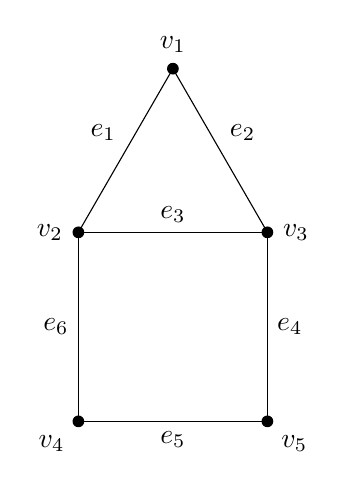
\begin{tikzpicture}[scale=1.2]
        \coordinate (v1) at (0,{1 + 1.732});
        \coordinate (v2) at (-1,1);
        \coordinate (v3) at (1,1);
        \coordinate (v4) at (-1,-1);
        \coordinate (v5) at (1,-1);

        \draw (v1) -- node[midway, above left] {$e_1$} (v2);
        \draw (v1) -- node[midway, above right] {$e_2$} (v3);
        \draw (v2) -- node[midway, above] {$e_3$} (v3);
        \draw (v3) -- node[midway, right] {$e_4$} (v5);
        \draw (v4) -- node[midway, below] {$e_5$} (v5);
        \draw (v2) -- node[midway, left] {$e_6$} (v4);

        \node[vertex, label=above:$v_1$] at (v1) {};
        \node[vertex, label=left:$v_2$] at (v2) {};
        \node[vertex, label=right:$v_3$] at (v3) {};
        \node[vertex, label=below left:$v_4$] at (v4) {};
        \node[vertex, label=below right:$v_5$] at (v5) {};
    \end{tikzpicture}
\end{center}

With the vertex order $(v_1,v_2,v_3,v_4,v_5)$ and the edge order $(e_1,e_2,e_3,e_4,e_5,e_6)$, the corresponding matrices are:
\[
A=
\begin{pmatrix}
0&1&1&0&0\\
1&0&1&1&0\\
1&1&0&0&1\\
0&1&0&0&1\\
0&0&1&1&0
\end{pmatrix}.
\]
\[
B=
\begin{pmatrix}
1&1&0&0&0&0\\
1&0&1&0&0&1\\
0&1&1&1&0&0\\
0&0&0&0&1&1\\
0&0&0&1&1&0
\end{pmatrix}.
\]
\[
D=
\begin{pmatrix}
2&0&0&0&0\\
0&3&0&0&0\\
0&0&3&0&0\\
0&0&0&2&0\\
0&0&0&0&2
\end{pmatrix}.
\]
\[
L=D-A=
\begin{pmatrix}
2&-1&-1&0&0\\
-1&3&-1&-1&0\\
-1&-1&3&0&-1\\
0&-1&0&2&-1\\
0&0&-1&-1&2
\end{pmatrix}.
\]

We can also verify the exercise $A=BB^T-D$ directly:
\[
BB^T=
\begin{pmatrix}
2&1&1&0&0\\
1&3&1&1&0\\
1&1&3&0&1\\
0&1&0&2&1\\
0&0&1&1&2
\end{pmatrix}.
\]
Hence
\[
BB^T-D=
\begin{pmatrix}
2&1&1&0&0\\
1&3&1&1&0\\
1&1&3&0&1\\
0&1&0&2&1\\
0&0&1&1&2
\end{pmatrix}
-
\begin{pmatrix}
2&0&0&0&0\\
0&3&0&0&0\\
0&0&3&0&0\\
0&0&0&2&0\\
0&0&0&0&2
\end{pmatrix}
=
\begin{pmatrix}
0&1&1&0&0\\
1&0&1&1&0\\
1&1&0&0&1\\
0&1&0&0&1\\
0&0&1&1&0
\end{pmatrix}
=A.
\]

\end{example}

\begin{definition}[$ k $-walk] 
Let $ G=(V,E) $ be a graph. A \emph{$ k $-walk} in $ G $ is a sequence of vertices $(v_0,v_1,\dots,v_k)$ such that $\{v_i,v_{i+1}\} \in E$ for all $ i=0,1,\dots,k-1 $. A walk is closed if $ v_0=v_k $. If a $ k $-walk is a path, then all vertices are distinct. If a $ k $-walk is a cycle, then all vertices are distinct except for the first and last vertices.  
\end{definition}

\chapter{Lecture 2}

引入 哥尼斯堡问题 一笔画问题 图一图二

\begin{definition} 
An Eulerian path is a walk which contains each edge of a graph exactly once. 
\end{definition}

\begin{definition} 
An Eulerian cycle is a closed Eulerian path. A graph is called Eulerian if it contains an Eulerian cycle.
\end{definition}

\begin{theorem} 
A finite connected graph is Eulerian if and only if every vertex has even degree.
\end{theorem}

\begin{proof} 
($ \Rightarrow $): If $ C=(x_0, \ldots, x_n) $ is an Eulerian cycle of $ G=(V,E) $ and a vertex $ y $ occurs $ t $ tinmes, then $ \deg (y)=2t $.

($ \Leftarrow $): Hierbolzer (1873). Algorithm: 

(1) Choose starting vertex $ x $.
\begin{itemize}
    \item take a walk from $ x $ without reusing $ x $  
    \item continue till stuck
    \item remove this walk with edges $ E_1 $, then graph $ (V,E \setminus E') $ still has only even degrees
    \item If $ E\setminus E' \neq \emptyset $, then repeat.
    \item If $ E\setminus E' = \emptyset $, then glue cycles together.
\end{itemize}
Complexity: $ O(|E|) $. 
\end{proof}

\begin{example} 
图3
\end{example}

\begin{definition} 
A Hamiltonion cycle is a closed walk which uses every vertex precisely once. A graph is called Hamiltonian if it contains a Hamiltonian cycle.
\end{definition}

If all degrees $ \ge \frac{n+1}{2}$, then $ G $ is Hamiltonian.

Random graphs are Hamiltonion. 

In general, problem of NP-complete.

P: det-turing machine can solve in polynomial time. NP: non-deterministic turing machine can solve in polynomial time.

NP-complete: any problem in NP can be reduced to an NP-complete in polynomial time.

Graph theory: structure graph theory, algorithmic graph theory, extremal graph theory\dots

Now we talk about trees.

\begin{definition} 
A connected graph with no cycles is called a tree.
\end{definition}

图4

\begin{definition} 
Disjoint unioin of trees is called forest.
\end{definition}

图5

\begin{definition} 
For a connected graph $ G=(V,E) $, a subgraph $ T=(V,E') $ a tree is called the spanning tree of $ G $.
\end{definition}

The spanning tree of $ G$ always exists.

\begin{theorem} 
The followings are equivalent:
\begin{enumerate}
\item $ G=(V,E) $ is a tree.
\item Any two vertices are connected by a unique path.
\item $ G $ is connected with $ |V|-1=|E| $.  
\end{enumerate}
\end{theorem}

\begin{proof} 
($ (1) \Rightarrow (2) $): If $ x,y $ are connected by two distinct paths, then we find a cycle.

($ (2) \Rightarrow (1) $): If $ G $ contains a cycle, then two vertices on the cycle are connected by two distinct paths. (The connectivity is clear).

($ (1) \Rightarrow (3) $): $ |V|=1 $, true. Now $ |V|>1 $, let $ P=(u,u_1, \ldots , u_l) $ be a longest path in $ G $, then all neighbors of $ u $ are in $ P $ and $ u $ must be a leaf. Remove the leaf, by induction we prove it.

()($ (3) \Rightarrow (1) $): $ G $ is connected so $ G $ has a spanning tree $ T $, then $ 1=|V(G)|-|E(T)| \ge |V(G)|-|E(G)|=1 $, hence $ E(G)=E(T) $ which implies $ G=T $ is a tree.     
\end{proof}

\begin{corollary}
$ G $ forest, $ \sharp $ connected components of $ G =|V(G)|-|E(G)|$ .  
\end{corollary}

\begin{corollary}
Let $ T $ be a tree, $ n:= |V(T)| \ge 2 $ with degree sequence $(d_1, \ldots, d_n)$. 图5 
\end{corollary}

What is the number of trees on n vertices? $ t(n) $. Cayley's formula.

图6

$ t(4)=16 $

\begin{theorem} 
$t(n)=n^{n-2} $. 
\end{theorem}

\begin{proof}
Goal: find a bijection between trees on sets $ [n] $ and $ [n]^{n-2} $.

Let $ T $ be a tree 

图7

\begin{enumerate}
\item $ u_1 \in u= \mathrm{min}\{ v \in V: \deg (v)=1  \} $, $ a_1 :=  $ unique neighbor of $ u_1 $.
\item Remove $ u_1 $ and repeat.    
\end{enumerate}

We get a sequence $ a=(a_1, \ldots, a_{n-2}) $ in $ [n]^{n-2} $. 

To show: For eah sequence $ a $ in $ [n]^{n-2} $, there is a unique tree $ T $.

Let $ \mathrm{d_i} := \sharp $ degree of vertex $ i $ and $ f_i := \sharp $ of occurabces of $ i $ in $ a $.

Note that $ f_i \le d_i -1 $ for all $ i $. Hence $ n-2=\sum f_i \le \sum (d_i-1)=(2n-2)-n =n-2 $. Hence $ f_i=d_i -1 $ for all $ i $. 

We construct $ T $: 
\begin{enumerate}
    \item Smallest $ b_1 $ not in $ (a_1,\ldots, a_{n-2}) $ and add edge $ (a_1,b_1) $  
    \item Take $ b_2 \neq  b_1 $ and  not in $ (a_2,\ldots, a_{n-2}) $ and add edge $ (a_2,b_2) $. Continue this processs any finially we construct a tree. 
\end{enumerate}
\end{proof}

\begin{proof} 
$ t(n: d_1, \ldots, d_n)=\sharp $ trees with degrees $ d_1, \ldots, d_n $.

Recall $ \binom{n}{r_1 \ldots r_k} = \sum_{i=1}^{n-1} \binom{n-1}{r_1 \ldots r_{i-1}r_{i+1}} \ldots r_k $.

Then $ t(n: d_1, \ldots, d_n)=\sum_{i=1}^{n} t(n-1: d_1, \ldots, d_{i-1}, d_{i+1}, \ldots, d_{n-1})$. WLOG, $ d_n=1 $ with basis $ t (3:d_1,d_2,d_3)=\binom{1}{d_1-1 d_2-1 d_3-1} $. We can prove $ t(n: d_1, \ldots, d_n)=\binom{n-2}{d_1-1 \ldots d_n-1} $. Using $ (x_1+ \ldots +x_k)^n=\sum \binom{n}{r_1 \ldots r_k} x_1^{r_1} \ldots x_k^{r_k} $, we get $ t(n)=n^{n-2} $    
\end{proof}

\begin{proof} 
Kirhoff's matrix tree theorem: $ \sharp  $ spanning trees of $ G $ is equal to $ \frac{1}{n} \cdot \lambda_1 \ldots \lambda_{n-1} $. Where $ \lambda_1, \ldots, \lambda_{n-1} $ non-zero eigenvalues of $ L(G) $. 

$ t(n)=\sharp $ spanning trees of $ K_n $. $ L(K_n)=nI-J $. Eigenvalues $ n-1 $ times $ n $, 1 times 0. Hence $ t(n)=\frac{1}{n} (n-1)^{n-1} =n^{n-2} $.
\end{proof}

see more proofs on your book.













\chapter{Homework}

\section{Week 1}

\begin{exercise}
Let $A$ be the adjacency matrix of a graph $G=(V, E)$.
\begin{enumerate}
    \item[(a)] Find a combinatorial interpretation for each entry of $A^2$ and $A^3$.
    \item[(b)] Show that $\operatorname{tr}\left(A^2\right)-2|E|$.
    \item[(c)] For $m \geq 2$ an integer, what does $\operatorname{tr}\left(A^m\right)$ count? Prove your claim.
\end{enumerate}
\end{exercise}

\begin{proof} 
\begin{enumerate}
\item[(a)] For $k\ge 1$ we have
\[
(A^k)_{ij}=\sum_{t_1,\dots,t_{k-1}} a_{i t_1}a_{t_1 t_2}\cdots a_{t_{k-1}j}.
\]
Each product $a_{i t_1}a_{t_1 t_2}\cdots a_{t_{k-1}j}$ equals $1$ precisely when
\[
v_i\sim v_{t_1}\sim v_{t_2}\sim \cdots \sim v_{t_{k-1}}\sim v_j,
\]
i.e.\ when $(v_i,v_{t_1},\dots,v_{t_{k-1}},v_j)$ is a walk of length $k$ from $v_i$ to $v_j$; otherwise the product is $0$.
Hence $(A^k)_{ij}$ counts the number of walks of length $k$ from $v_i$ to $v_j$.

In particular:
\[
(A^2)_{ij}=\sum_{t=1}^n a_{it}a_{tj}
\]
counts the number of vertices $v_t$ adjacent to both $v_i$ and $v_j$, i.e.\ the number of length-$2$ walks $v_i\to v_t\to v_j$.

Similarly,
\[
(A^3)_{ij}=\sum_{s,t=1}^n a_{is}a_{st}a_{tj}
\]
counts the number of length-$3$ walks $v_i\to v_s\to v_t\to v_j$.

\item[(b)] Since $a_{ii}=0$ for a simple graph, we have
\[
(A^2)_{ii}=\sum_{t=1}^n a_{it}a_{ti}=\sum_{t=1}^n a_{it}^2=\sum_{t=1}^n a_{it}=\deg(v_i).
\]
Therefore
\[
\operatorname{tr}(A^2)=\sum_{i=1}^n (A^2)_{ii}=\sum_{i=1}^n \deg(v_i).
\]
By the Handshaking Lemma, $\sum_{i=1}^n \deg(v_i)=2|E|$. Hence
\[
\operatorname{tr}(A^2)=2|E|
\quad\text{(equivalently, }\operatorname{tr}(A^2)-2|E|=0\text{).}
\]

\item[(c)] For any integer $m\ge 1$, by the argument in (a),
\[
(A^m)_{ij}\ \text{counts the number of walks of length $m$ from $v_i$ to $v_j$}.
\]
In particular, $(A^m)_{ii}$ counts the number of \emph{closed} walks of length $m$ starting and ending at $v_i$.
Summing over $i$ yields
\[
\operatorname{tr}(A^m)=\sum_{i=1}^n (A^m)_{ii},
\]
so $\operatorname{tr}(A^m)$ counts the total number of closed walks of length $m$ in $G$, where a closed walk is counted with its chosen starting vertex (i.e.\ each closed walk contributes $1$ to exactly one diagonal entry, the entry corresponding to its start/end vertex).
\end{enumerate}
\end{proof}

\begin{exercise}
The girth of a graph $G$ is the length of the smallest polygon in the graph. Let $G$ be a graph of girth 5 for which all vertices have degree at least $d$. Show that $G$ has at least $d^2+1$ vertices. Can equality hold?
\end{exercise}

\begin{proof}
Fix a vertex $x\in V(G)$ and write $N(x)=\{y_{1},\dots,y_{t}\}$ as the set of neighbors of $x$, where $t=\deg(x)\ge d$.

\noindent\emph{Step 1: no triangles.}
Since the girth is $5$, $G$ has no $3$-cycles. Hence the neighbors of $x$ are pairwise nonadjacent:
$y_i\not\sim y_j$ for $i\neq j$.

\noindent\emph{Step 2: no $4$-cycles.}
Again girth $5$ implies there is no $4$-cycle. Thus if $z\neq x$ were adjacent to both $y_i$ and $y_j$
for $i\neq j$, then $x-y_i-z-y_j-x$ would be a $4$-cycle, a contradiction. Therefore the sets
\[
N(y_i)\setminus\{x\}\qquad (i=1,\dots,t)
\]
are pairwise disjoint.

\noindent\emph{Step 3: counting.}
All vertices in
\[
\{x\}\ \cup\ N(x)\ \cup\ \bigcup_{i=1}^{t}\bigl(N(y_i)\setminus\{x\}\bigr)
\]
are distinct, so
\[
|V(G)|\ \ge\ 1+t+\sum_{i=1}^{t}\bigl|N(y_i)\setminus\{x\}\bigr|
\ =\ 1+t+\sum_{i=1}^{t}\bigl(\deg(y_i)-1\bigr).
\]
Since $\deg(y_i)\ge d$ for all $i$, we get $\deg(y_i)-1\ge d-1$, hence
\[
|V(G)|\ \ge\ 1+t+t(d-1)\ =\ 1+td\ \ge\ 1+d^{2}.
\]
This proves $|V(G)|\ge d^{2}+1$.

\noindent\emph{Step 4: the equality case.}
If $|V(G)|=d^{2}+1$, then all inequalities above are tight. In particular, $\deg(x)=t=d$ and
$\deg(y_i)=d$ for all $i$. Repeating the argument with $x$ replaced by an arbitrary vertex shows that
$G$ is $d$-regular. Tightness also forces that every vertex $z\notin \{x\}\cup N(x)$ is adjacent to
\emph{exactly one} neighbor of $x$ (otherwise we would either miss vertices or create a $4$-cycle).
Equivalently, any two nonadjacent vertices have exactly one common neighbor, while adjacent vertices
have none (otherwise a triangle would appear). Hence $G$ is strongly regular with parameters
\[
(v,k,\lambda,\mu)=(d^{2}+1,\ d,\ 0,\ 1).
\]
Such graphs are precisely the Moore graphs of girth $5$.

\noindent\emph{Step 5: why $d=4$ cannot have equality.}
Assume for contradiction that equality holds for $d=4$. Then $G$ would be strongly regular with
\[
(v,k,\lambda,\mu)=(17,4,0,1).
\]
For a strongly regular graph, the two nontrivial adjacency eigenvalues are
\[
r,s=\frac{(\lambda-\mu)\pm\sqrt{(\lambda-\mu)^{2}+4(k-\mu)}}{2},
\]
and their multiplicities are
\[
m_r=\frac12\left((v-1)-\frac{2k+(v-1)(\lambda-\mu)}{\sqrt{\Delta}}\right),\qquad
m_s=\frac12\left((v-1)+\frac{2k+(v-1)(\lambda-\mu)}{\sqrt{\Delta}}\right),
\]
where $\Delta=(\lambda-\mu)^{2}+4(k-\mu)$.
Substituting $(v,k,\lambda,\mu)=(17,4,0,1)$ gives $\Delta=13$ and
$2k+(v-1)(\lambda-\mu)=8+16(-1)=-8$, hence
\[
m_r=\frac12\left(16+\frac{8}{\sqrt{13}}\right),\qquad
m_s=\frac12\left(16-\frac{8}{\sqrt{13}}\right),
\]
which are not integers. This contradicts that eigenvalue multiplicities must be integers.
Therefore no such graph exists, and equality cannot hold when $d=4$.
\end{proof}

\begin{remark}
Known examples achieving $|V(G)|=d^{2}+1$ occur for $d=2$ (the cycle $C_{5}$),
$d=3$ (the Petersen graph), and $d=7$ (the Hoffman--Singleton graph). A hypothetical case $d=57$
is a famous open problem; for all other $d$ equality is impossible.
\end{remark}

\begin{exercise}
Let $Q=\{1, \ldots, q\}$ be the graph with vertex set $Q^n$, two vertices adjacent if they differ in exactly one coordinate. Show that $Q$ is Hamiltonian.
\end{exercise}

\begin{definition}[Hamiltonian graph]
A (finite) graph $G=(V,E)$ is called \emph{Hamiltonian} if it contains a \emph{Hamiltonian cycle},
i.e., there exists a cycle that visits every vertex of $G$ exactly once (except that the starting
vertex is repeated at the end).
Equivalently, $G$ is Hamiltonian if there exist distinct vertices
$v_1,\dots,v_n\in V$ with $n=|V|$ such that
\[
\{v_i,v_{i+1}\}\in E \ \text{for } i=1,\dots,n-1,
\qquad\text{and}\qquad
\{v_n,v_1\}\in E .
\]
\end{definition}

\begin{exercise}
Find the six nonisomorphic trees on 6 vertices, and for each compute the number of distinct spanning trees in $K_6$ isomorphic to it.
\end{exercise}

\begin{exercise}
\begin{enumerate}
    \item[(a)] Suppose a tree $G$ has exactly one vertex of degree $i$ for $2 \leq i \leq m$ and all other vertices have degree 1 . How many vertices does $G$ have?
    \item[(b)] Suppose a tree $G$ ha exactly one vertex of degree $i$ for $2 \leq i \leq m$ and $k$ other vertices have degree 1 . Prove that $k \geq\left[\frac{m+3}{2}\right]$ and give a construction for such a graph.
\end{enumerate}
\end{exercise}













\end{document}
